\newpage{\ } 
\thispagestyle{empty} 

\chapter{Cambio Clim\'atico}
\lhead{Capítulo 2. \emph{Cambio Clim\'atico}} % This is for the header on each page - perhaps a shortened title


El cambio clim\'atico es definido como cualquier variaci\'on del clima a lo largo del tiempo, ya sea por variabilidad natural o como resultado de las actividades humanas que altera la composici\'on de la atm\'osfera y que se suma a la variabilidad clim\'atica natural observada en periodos de tiempos comparables \cite{robert2002captura}.\\~\\
En la Figura \ref{fig:cambioClimatico} podemos observar como el planeta tierra esta cubierta por una capa de gases que deja penetrar energ\'ia solar que calienta la superficie terrestre. Algunos de los gases en la atm\'osfera, llamados gases de efecto invernadero (GEI), impiden el escape de este calor hacia el espacio . El escape de calor  mantiene a la tierra a una temperatura promedio arriba del punto de congelaci\'on del agua y permite la vida. A pesar de esto, las actividades humanas est\'an produciendo un exceso de gases que est\'an potencialmente calentando el clima de la tierra \cite{almando2014estimacion}.
    \begin{figure}[!hbtp]
    	\centering
    	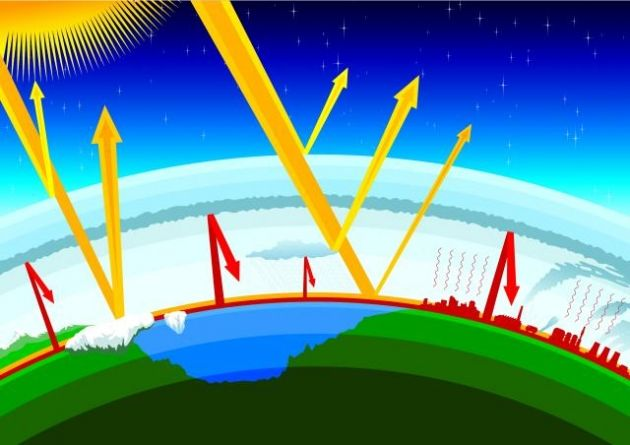
\includegraphics[width=0.5	\textwidth]{./Figures/cap2/calentamientoGlobal.jpg}
    	\caption{Calentamiento Global \cite{calent2015global}.}
    	\label{fig:cambioClimatico}
    \end{figure}


\section{Ciclo de carbono} 
Las plantas absorben el dióxido de carbono existente en el aire o el agua, acumul\'andolos en los tejidos vegetales en forma de materia org\'anica, mediante la fotos\'intesis \cite{natur2015PW}. Posteriormente, los animales herb\'ivoros se alimentan de estos vegetales para transferir esa energ\'ia a los dem\'as niveles (carnívoros que se alimentan de los herb\'ivoros).
La energía transferida sigue varios caminos: por un lado es devuelto a la atm\'osfera como di\'oxido de carbono mediante la respiraci\'on; por otro lado se deriva hacia el medio acu\'atico, donde puede quedar como sedimentos org\'anicos, o combinarse con las aguas para producir carbonatos y bicarbonatos (suponen el 71\% de los recursos de carbono de la Tierra). La acumulaci\'on de carbono en zonas h\'umedas genera turba (carb\'on ligero y esponjoso), resultado de una descomposición incompleta, lo que da lugar a la formaci\'on de dep\'ositos de combustibles f\'osiles como petr\'oleo, carb\'on y gas natural.\\~\\
El ciclo del carbono queda completado gracias a los organismos des\-componedores, los cuales llevan a cabo el proceso de mineralizar y descomponer los restos org\'anicos, cad\'averes, excrementos, entre otros. Adem\'as de la actividad que llevan a cabo el reino vegetal y animal en el ciclo, tambi\'en liberan carbono la putrefacci\'on y la combusti\'on \cite{natur2015PW}. La Figura \ref{fig:ciclocarbono} nos presenta el ciclo completo del carbono.
    \begin{figure}[!hbtp]
    	\centering
    	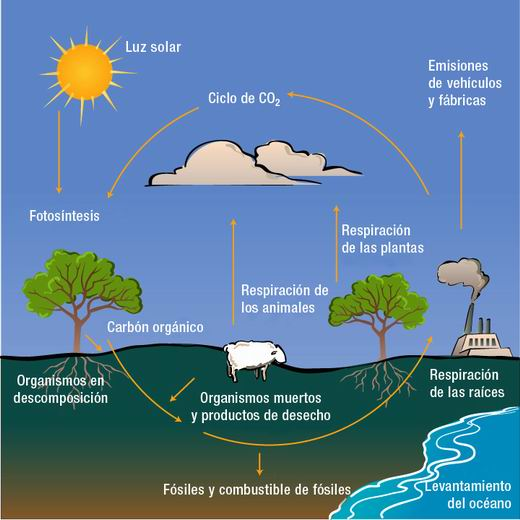
\includegraphics[width=0.5	\textwidth]{./Figures/cicloCarbono.jpg}
    	\caption{Ciclo de carbono \cite{ciclot2015carbo}.}
    	\label{fig:ciclocarbono}
    \end{figure}


\subsection{Secuestro de carbono}
El CO2 y otros gases invernaderos actúan atrapando la energ\'ia cal\'orica (radiación solar de onda corta) reflejada de la superficie de la tierra y las nubes \cite{encaptura}. Este calor retenido puede conducir al calentamiento global en el planeta. Los niveles del di\'oxido de carbono atmosf\'erico pueden reducirse en la misma medida que los niveles de carbono org\'anico del suelo aumentan a trav\'es del secuestro de carbono. Si el carbono org\'anico del suelo no es alterado, puede permanecer en el suelo por muchos a\~{n}os como materia org\'anica estable. Este carbono es entonces secuestrado o removido de la atm\'osfera para ser reciclado. De esta forma se pueden reducir los niveles de CO2, disminuyendo las probabilidades de calentamiento global \cite{castillo2003manejo}.
\subsection{P\'erdida de Carbono}
P\'erdida de carbono se refiere a aquella porci\'on de carbono que no pudo ser almacenada o capturada en el intercambio normal que ocurre entre la superficie terrestre y la atm\'osfera en el ciclo de carbono \cite{marquezestimacion}, contribuyendo al calentamiento global mediante la emisión de di\'oxido de carbono que compone el grupo de gases de efectos invernaderos.
\subsection{Secuestro de carbono en Paraguay}
El Fondo para el Medio Ambiente Mundial (FMAM) y el Programa de Peque\~{n}as Donaciones (PDD), en nuestro pa\'is, nos dice que el uso de hidrocarburos para generar energ\'ia el\'ectrica, el uso de biomasa como fuente de energ\'ia, las emisiones industriales, la deforestaci\'on, los incendios forestal, la actividad pecuaria, el manejo y disposici\'on de residuos y la actividad del transporte son los que presentan mayores emisiones de carbono \cite{cecilia2010Proyecto}, en consecuencia contribuyen al cambio clim\'atico.
\subsection{Gran Chaco Americano}
En el territorio del Gran Chaco Americano, se detecta una tendencia de importante aumento de las tasas de deforestaci\'on diaria por encima de las 1.400 hect\'areas, siendo el promedio del per\'iodo 15 de junio al 10 de julio de 2.011, de 1.042 hect\'areas por d\'ia, y del per\'iodo 10 de julio al 13 de agosto de 2.011 de 1.408 hect\'areas por d\'ia en toda la regi\'on, dando un total de 47.856 hect\'areas de \'areas boscosas que registraron cambio a uso agropecuario, en 34 d\'ias. Entre los pa\'ises que componen el Gran Chaco Americano,  Paraguay  registr\'o el mayor porcentaje de la deforestaci\'on (86\%), seguido por Argentina (13\%) y Bolivia (1\%). En Brasil, no se detectaron caso de deforestaci\'on para la regi\'on. En el caso espec\'ifico de Paraguay, la tasa de deforestaci\'on diaria ha aumentado, pasando de 998 hect\'areas por d\'ia a 1.210 hect\'areas por d\'ia \cite{fao2003revista}, perdi\'endose por consiguiente en gran medida sumideros de carbono, lo cual va aportando al desequilibrio del ciclo. En la Tabla \ref{tab:chacoamericano} podemos observar los principales problemas ambientales que afronta el Gran Chaco Americano, en cada pa\'is que lo compone.
\begin{table}[!hbtp]
	\centering
	\caption{Problem\'atica que afrontan los países del gran chaco americano \cite{gustavo2012deteccion}.}
	\label{tab:chacoamericano}
	\begin{tabular}{|p{4cm}|p{4cm}|p{4cm}|}
		\hline
		{\bf Argentina} & {\bf Bolivia} & {\bf Paraguay} \\ \hline
		Deforestaci\'on de los bosques nativos. & Deforestaci\'on de los bosques nativos. & Deforestaci\'on de los bosques nativos. \\ \hline
		Excesiva dependencia dela producci\'on ganadera y explotaci\'on forestal. & Sobrepastoreo. & Sobrepastoreo. \\ \hline
		Sobrepastoreo. & Incendios de bosques y pastizales. & Incendios de bosques y pastizales. \\ \hline
		Incendios de bosques y pastizales. & P\'erdida de biodiversidad. & Manejo no sustentable de los recursos h\'idricos. \\ \hline
		Perdida de labiodiversidad. & Cambio clim\'atico. & P\'erdida de biodiversidad. \\ \hline
		Cambio clim\'atico. &  & Cambio clim\'atico. \\ \hline
	\end{tabular}
\end{table}


\section{Biomasa}
La biomasa es aquel material org\'anico biodegradable y no fosilizado originado de plantas, animales y microorganismos; incluye productos, subproductos, residuos y desechos de la agricultura, forester\'ia e industrias afines, as\'i como las fracciones org\'anicas y no fosilizadas de los desechos industriales y municipales. La biomasa tambi\'en incluye los gases y l\'iquidos recuperados de la descomposici\'on de materiales org\'anicos biodegradables y no fosilizados \cite{salinas2008guia}.
La biomasa es considerada como la masa total de organismos vivos en una zona o volumen determinado (a menudo también se incluyen los restos de plan que han muerto recientemente). La cantidad de biomasa se expresa mediante su peso en seco o su contenido de energ\'ia de carbono o de nitr\'ogeno \cite{garciduenas1987produccion}.
\subsection{Biomasa Forestal}
La biomasa forestal se define como el peso (o estimaci\'on equivalente) de materia org\'anica que
se encuentra en un determinado ecosistema forestal por encima y por debajo del suelo \cite{schlegel2000manual}, normalmente es
cuantificada en toneladas por hect\'area de peso verde o seco. La biomasa forestal es frecuentemente separada en
componentes, donde los m\'as t\'ipicos corresponden a la masa del fuste, ramas, hojas, corteza,
ra\'ices, hojarasca y madera muerta. \\~\\
En t\'erminos de p\'erdida y secuestro, representa la cantidad potencial de carbono que puede ser liberada a la atm\'osfera, debida a la deforestaci\'on, o la conservada en superficies terrestres cuando los bosques son correctamente gestionados \cite{lu2005exploring}.

\section{Medici\'on de balances de carbono}
La din\'amica del balance de carbono en un ecosistema forestal es muy compleja de medir, ya que es necesario determinar la captura de carbono por crecimiento de biomasa en los \'arboles y otros componentes en la vegetaci\'on como las p\'erdidas ocasionadas por disturbios, sean naturales o por actividades humanas; descomposici\'on de madera muerta; y la transferencia entre los compartimentos vivos, muertos y el suelo \cite{angelsen2008moving}.\\~\\
Existen metodolog\'ias que permiten medir y monitorear cambios en reservorios promedios de carbono por unidad de \'area. A continuaci\'on se citan algunos de ellos:

\begin{itemize}
	
	\item \textbf{Inventarios forestales:} se establecen relaciones alom\'etricas con mediciones de terreno en funci\'on al di\'ametro o volumen de arboles con las reservas de carbono forestal. La desventaja que presenta es su lentitud al realizar en \'areas grandes y costo elevado que presenta \cite{asner2005selective}. Definiendo alom\'etria como los cambios de dimensi\'on relativa de las partes corporales correlacionados con los cambios en el tama\~{n}o total. 
	\item \textbf{Sensores remotos:} existen diferentes tipos de sensores que permiten monitorear cambios en reservorios de carbono vegetal con mayor dinamismo y a gran escala \cite{libro2012Tsuyuki}. Podemos citar:
	\begin{enumerate}
	\item \textbf{Sensores remotos \'opticos (pasivos):} capturan luz solar o artificial reflejada desde el objeto, detectando la intensidad de luz visible e infrarroja en una o mas longitudes de ondas.
	\item  \textbf{Sensores remotos activos:} este sensor se encuentra montado en un sat\'elite, el cual emite pulsos de microondas oblicuamente detectando y registrando la intensidad, fase y tiempo de los impulsos reflejados desde la superficie terrestre.
	\item  \textbf{Sensores remotos l\'aser como LiDAR (detecci\'on \'area de luz y medidas de rango):} mide la distancia entre el sensor y el objeto usando el tiempo que tarda el pulso en viajar y la intensidad del pulso reflejado del objeto.
	\end{enumerate}
	La Figura \ref{fig:sensores} nos muestra como la informaci\'on es capturada, por medio de los 3 tipos de sensores descriptos.  
	    \begin{figure}[!hbtp]
	    	\centering
	    	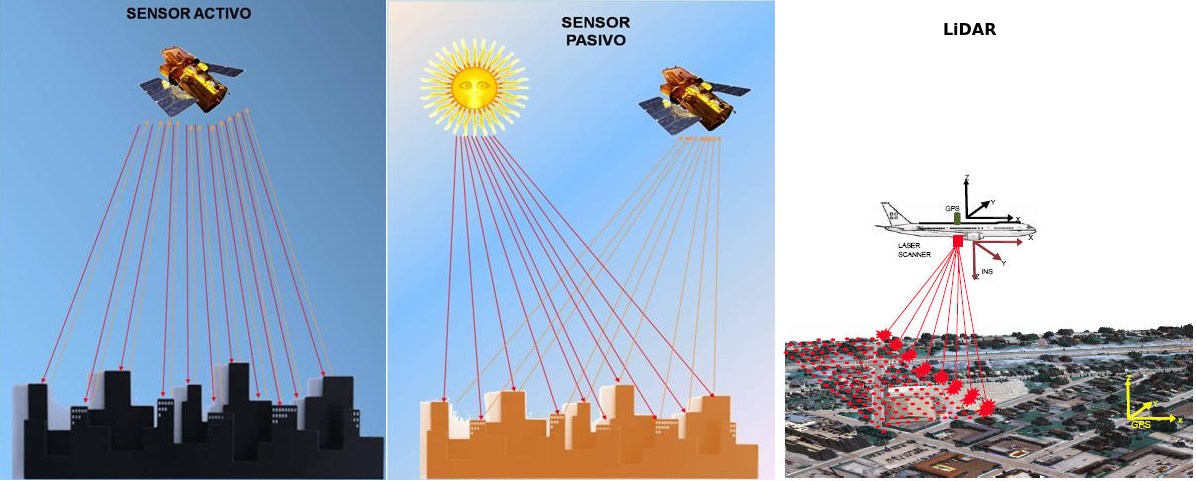
\includegraphics[width=0.9	\textwidth]{./Figures/sensores.png}
	    	\caption{Tipos de sensores.}
	    	\label{fig:sensores}
	    \end{figure}
\end{itemize}

\section{Teledetecci\'on en el medio ambiente}
El t\'ermino teledetecci\'on esta definida como la ciencia y arte de obtener informaci\'on referente a la superficie terrestre sin entrar en contacto con ella. Esto se realiza detectando y grabando la energ\'ia emitida o reflejada para su procesamiento, an\'alisis y aplicaci\'on de esa informaci\'on \cite{salinero2002teledeteccion}.\\~\\
En los \'ultimos a\~{n}os se han desarrollado bastantes aplicaciones en casi todas las \'areas que involucra la tierra, debido a las grandes posibilidades y ventajas que presenta con la localizaci\'on de espacios geogr\'aficos, observaci\'on de fen\'omenos temporales e integraci\'on de resultados a los sistemas de informaci\'on geogr\'afica, reduciendo los costos en dinero y tiempo empleados en estudios sobre el terreno \cite{baker2006mapping}. La aplicaci\'on de la teledetecci\'on en los recursos naturales se fundamenta en que los elementos del mismo tienen un respuesta espectral propia a los sensores remotos. Por ello, la teledetecci\'on espacial es empleada como complemento y no como sustituto a estudios ambientales por permitir realizarlos a escalas espaciales y temporales distintas a las que se acceden desde experimentos controlados, lo cuales son tambi\'en necesarios e imprescindibles pero a veces insuficientes \cite{perez2011aplicaciones}.\\~\\
En la Figura \ref{fig:tele} podemos observar el proceso completo de la teledetecci\'on. El sensor remoto montado en el satelite captura la informaci\'on terrestre por medio de la energ\'ia solar. En una estaci\'on de recepci\'on, la informaci\'on capturada es transformada a im\'agenes para poder ser procesadas por el hombre en alg\'un tipo de an\'alisis. 

	\begin{figure}[H]
		\centering
		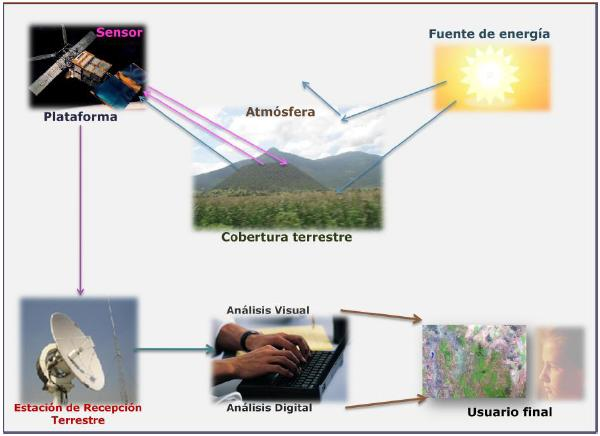
\includegraphics[width=0.7	\textwidth]{./Figures/cap3/teledeteccion.png}
		\caption{Teledetecci\'on \cite{teledet2015perce}.}
		\label{fig:tele}
	\end{figure}

\section{Resumen}

La perdida de los bosques provocan da\~{n}os con consecuencias exponenciales al medio ambiente, ya que representan un factor fundamental en la estabilidad clim\'atica de la tierra. Las tierra esta cubierta por gases que dejan penetrar la energ\'ia solar, manteniendo temperaturas optimas para la vida. Algunos de los gases impiden el escape del calor hacia el espacio, a estos gases se los llaman gases de Efecto Invernadero (GEI). Las actividades humanas producen en exceso los GEI, principalmente con di\'oxido de carbono (CO2) a trav\'es de la deforestaci\'on y degradaci\'on en los bosques. La fotos\'intesis compone un elemento fundamental en el proceso natural denominado ciclo del carbono, mitigando el CO2 de la atm\'osfera con transformaciones del gas a materia org\'anica en las plantas (biomasa), a esto se lo conoce como secuestro de carbono. El chaco paraguayo presenta una tendencia importante en el aumento de las tasas de deforestaci\'on, siendo entre los pa\'ises que componen el Gran chaco americano el que presenta mayor porcentaje (86\%). 
En el 2011, el chaco paraguayo registro un promedio diario de 1402 hect\'areas de bosques deforestados a causa de actividades humanas ligadas a la agricultura, silvicultura y ganadería, por ello la medici\'on del balance de carbono en nuestro pa\'is resulta importante para controles del manejo del medio ambiente. Los inventarios forestales establecen relaciones entre reservas de carbono forestal y variables alom\'etricas de los arboles  para medir el contenido de carbono, presentando como principal dificultad la lentitud en el estudio de \'areas extensas. En cambio, el empleo de procesamiento digital de im\'agenes satelitales junto con la teledetecci\'on nos brindan un dinamismo en el monitoreo a gran escala.